   \begin{center}
      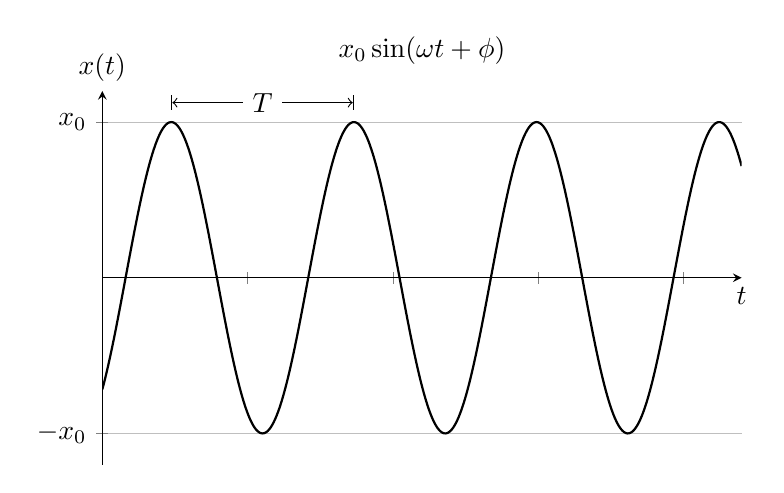
\begin{tikzpicture}

         \def\dx{0.8}

         \begin{axis}[
            width = 0.8\textwidth,
            height = 15\baselineskip,
            axis lines= middle, 
            xlabel=$t$, 
            every axis x label/.style={at={(current axis.right of origin)}, anchor=north},
            every axis y label/.style={at={(current axis.north west)}, anchor=south},
            ylabel=$x(t)$, 
            title={$x_0 \sin(\omega t + \phi)$}, 
            ymin = -1.2, 
            ymax = 1.2,
            ytick={1,-1},
            yticklabels={$x_0$, $- x_0$},
            ymajorgrids,
            xtick={},
            xticklabels={},
            ]

            
            \addplot[domain=-0:7*pi, samples=500, thick]{sin(deg(x - \dx))};
            \draw[|<->|] (axis cs: 0.5*pi + \dx, 1.125) -- node[fill=white]{$T$} (axis cs: 2.5*pi + \dx, 1.125);

         \end{axis}
      \end{tikzpicture}
   \end{center}
